\documentclass{article}

\usepackage{polski}
\usepackage[utf8]{inputenc}
\usepackage{graphicx}
\usepackage{float}
\usepackage{amsmath}
\usepackage{geometry} 

\author{Jakub Postępski}
\title{STP - Projekt, zadanie 1.2}
\begin{document}
\maketitle

Obiekt opisany jest transmitancją ciągłą
\[ G(s) = \frac{0.5s^2 +3.25s+5.25}{s^3 +7s^2 -14s-120} \]
\section{Zadanie 1}
\subsection{Transmitancja dyskretna}
Transmitancja dyskretna została wyliczona przy użyciu Matlaba.
Najpierw użyto polecenia \textit{tf}, które tworzy model transmitancji wykorzystywany do obliczania transmitancji dyskretnej. 
\[G = tf(\begin{bmatrix}0.5& 3.25& 5.25],&[1& 7& -14& -120\end{bmatrix})\]

Do wyliczania z modelu transmitancji dyskretnej użyto polecenia \textit{c2d}.
\[Gd = c2d(G,0.1,'zoh')\]

Transmitancja dyskretna obiektu ma następującą postać:
\[ G(z) = \frac{0.05095 z^2 - 0.07384 z + 0.02672}{z^3 - 2.647 z^2 + 2.056 z - 0.4966} \]

\subsection{Zera i bieguny transmitancji}
Korzystając z funkcji \textit{roots} dostajemy:
\begin{itemize}
\item zera transmitancji ciągłej: $s_0=-3.5$; $s_1=-3$
\item bieguny transmitancji ciągłej: $s_{00}=-6$; $s_{01}=-5$; $s_{02}=4$
\item zera transmitancji dyskretnej: $s_0=0.6990$; $s_1=0.7502$
\item bieguny transmitancji dyskretnej: $s_{00}=0.5529$; $s_{01}=0.6019$; $s_{02}=1.4922$
\end{itemize}
Obiekt jest nie jest stabilny, ponieważ wszyskie bieguny transmitancji ciągłej nie znajdują się w lewej półpłaszczyźnie, co jest warunkiem stabilności asymptotycznej. Dla transmitancji dyskretnej obiekt nie jest stabilny, bo wszystkie nie wszyskie bieguny mają wartość bezwzględną mniejszą od 1, co jest warunkiem stabilności asymptotycznej.
\section{Zadanie 2}
\subsection{Pierwszy wariant metody bezpośredniej}
Licznik oraz mianownik wyliczonej wcześniej transmitancji dyskretnej mnożymy przez $z^{-3}$ otrzymując:
\[ G(z)= \frac{Y(z)}{U(z)}= \frac{0.05095 z^{-1} - 0.07384z^{-2} + 0.02672}{1 - 2.647z^{-1} + 2.056z^{-2} - 0.4966z^{-3}} \]
i wprowadzamy sygnał pomocniczy:
\[E(z) = \frac{U(z)}{1 - 2.647z^{-1} + 2.056z^{-2} - 0.4966z^{-3}}\]
więc:
\[E(z) = U(z)-(- 2.647z^{-1} + 2.056z^{-2} - 0.4966z^{-3})E(s)\]
\[Y(z) = (0.05095 z^{-1} - 0.07384z^{-2} + 0.02672)E(z) \]
Otrzymujemy reprezentację macierzową, oraz reprezentację graficzną (rysunek \ref{wariant1}):
\[A_1=\begin{bmatrix}
-2.647 & 2.056 & -0.4996 \\ 1 & 0 & 0 \\ 0 & 1 & 0
\end{bmatrix}\]
\[B_1=\begin{bmatrix}
1 \\ 0 \\ 0
\end{bmatrix}\]
\[C_1=\begin{bmatrix}
0.05095 & -0.07384 & 0.00267
\end{bmatrix}\]
\[D_1 = 0\]
\begin{figure}[h]
\centering
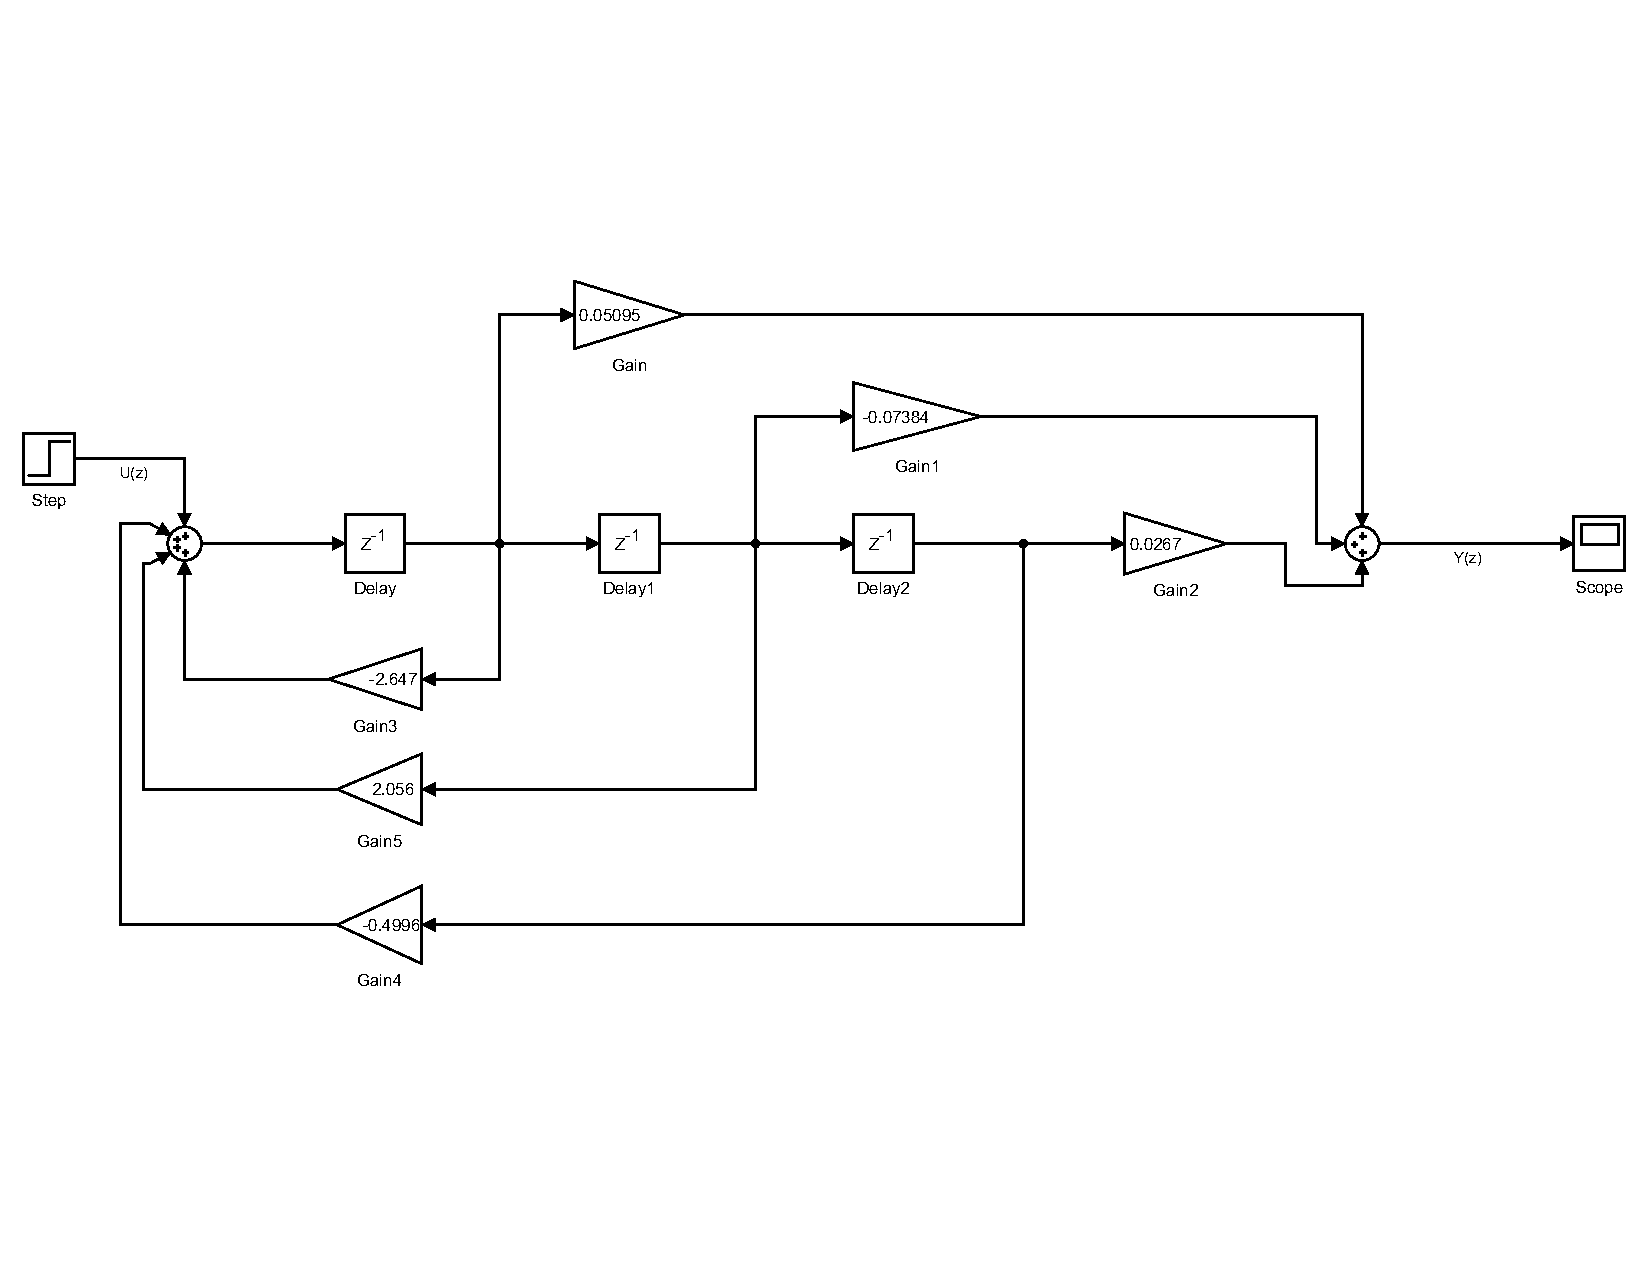
\includegraphics[width=0.8\linewidth]{wariant1}
\caption{Reprezentacja modelu dyskretnego, w wariancie pierwszym metody bezpośredniej}
\label{fig:wariant1}
\end{figure}
\subsection{Drugi wariant metody bezpośredniej}
Korzystając z zależności:
\[A_2 = A_1^T, B_2 = C_1^T, C_2 = B_1^T, D = 0\]
otrzymujemy reprezentację macierzową i reprezentację graficzną (rysunek \ref{wariant2}):
\[A_2=\begin{bmatrix}
-2.647 & 1 & 0 \\ 2.056 & 0 & 1 \\ -0.4996 & 0 & 0
\end{bmatrix}\]
\[B_2=\begin{bmatrix}
0.05095 \\ -0.07384 \\ 0.00267
\end{bmatrix}\]
\[C_2=\begin{bmatrix}
1 & 0 & 0
\end{bmatrix}\]
\[D_2 = 0\]
\begin{figure}[h]
\centering
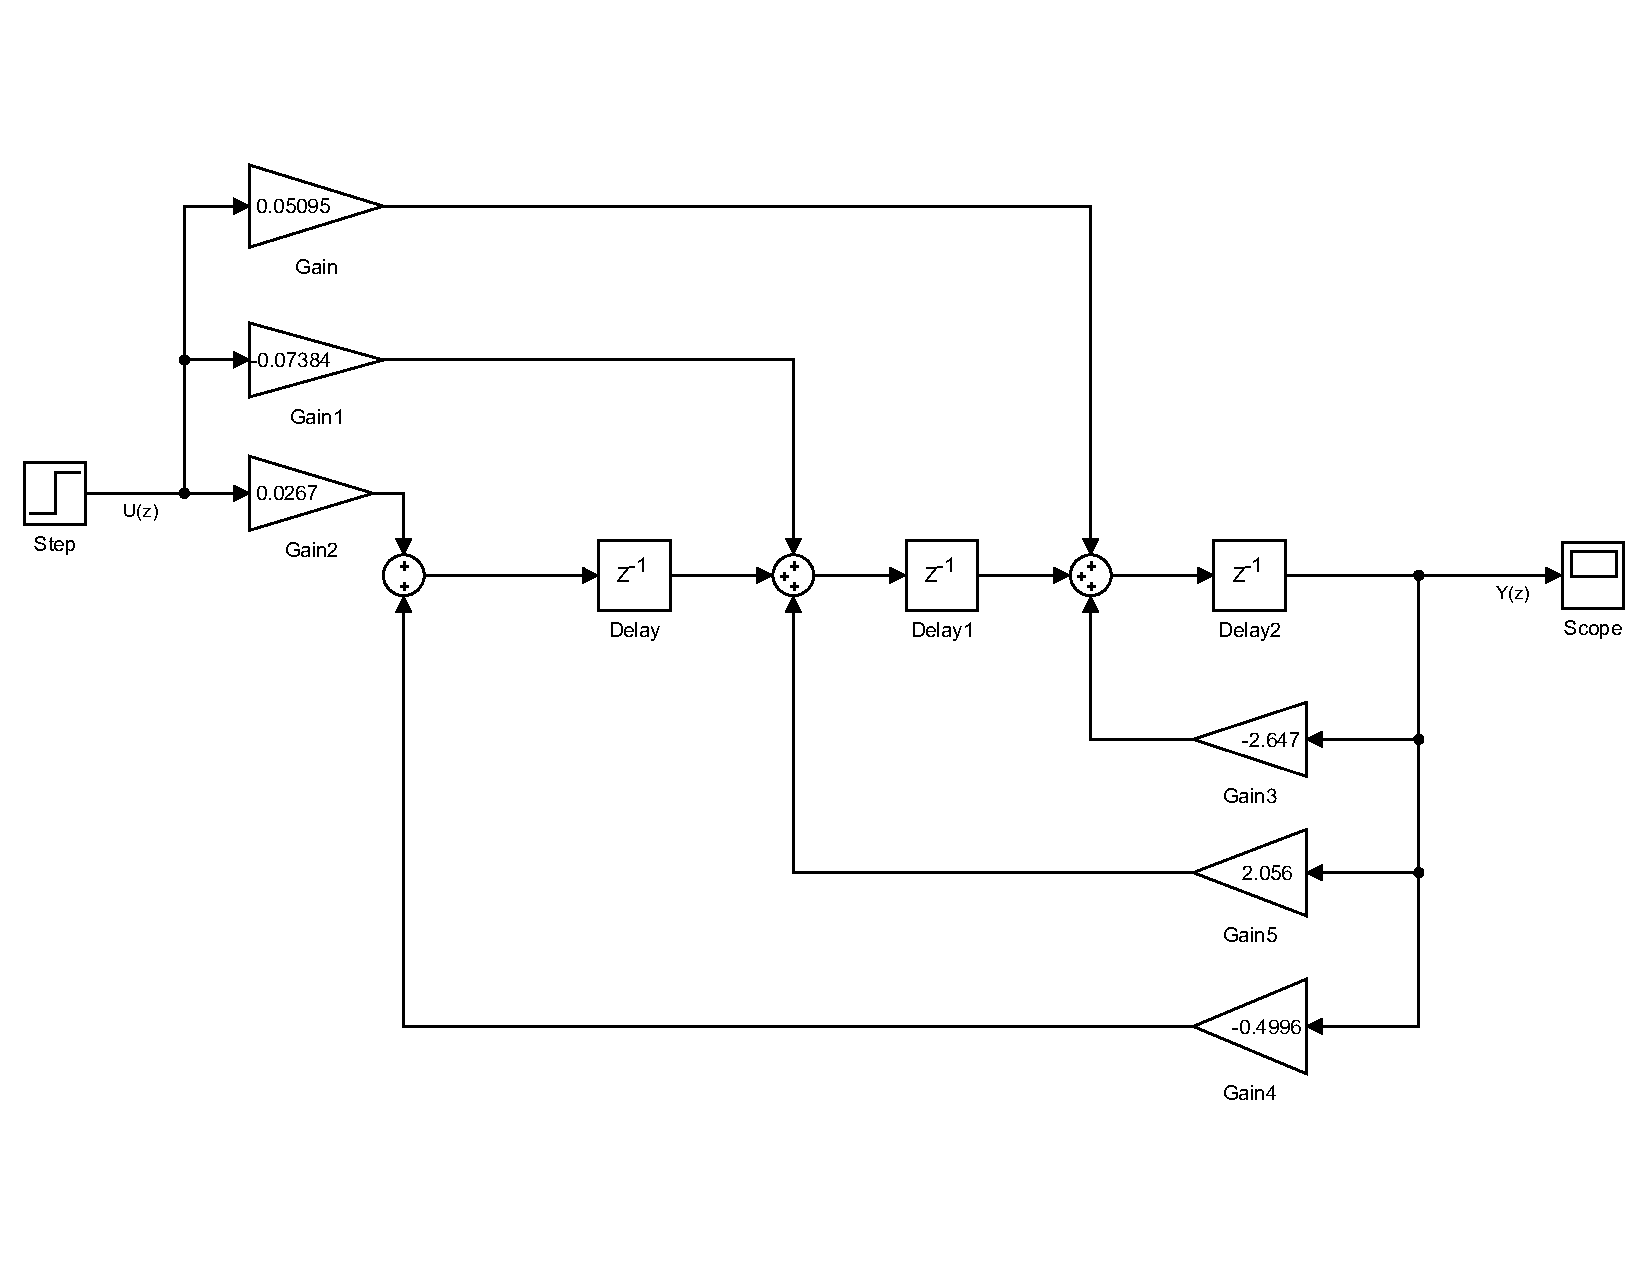
\includegraphics[width=0.8\linewidth]{wariant2}
\caption{Reprezentacja modelu dyskretnego, w wariancie drugim metody bezpośredniej}
\label{fig:wariant2}
\end{figure}
\section{Zadanie 3}
Wyznaczamy wektor sprzężeń zwrotnych K. Rozwiązujemy równianie charakterystyczne:
\[|zI -(A-BK) = (z-z_1)(z-z_2)(z-z_3)|\]
Do wyliczania wektorów K zastosowano funkcję \textit{acker()}.
Układ wykorzystany w zadaniu przedstawia rysunek
\subsection{Wyliczanie wektora K dla równych biegunów}

\end{document}